\upaper{12}{The Universe of Universes}
\uminitoc{Space Levels of the Master Universe}
\uminitoc{The Domains of the Unqualified Absolute}
\uminitoc{Universal Gravity}
\uminitoc{Space and Motion}
\uminitoc{Space and Time}
\uminitoc{Universal Overcontrol}
\uminitoc{The Part and the Whole}
\uminitoc{Matter, Mind, and Spirit}
\uminitoc{Personal Realities}
\author{Perfector of Wisdom}
\vs p012 0:1 The immensity of the far\hyp{}flung creation of the Universal Father is utterly beyond the grasp of finite imagination; the enormousness of the master universe staggers the concept of even my order of being. But the mortal mind can be taught much about the plan and arrangement of the universes; you can know something of their physical organization and marvellous administration; you may learn much about the various groups of intelligent beings who inhabit the seven superuniverses of time and the central universe of eternity.
\vs p012 0:2 In principle, that is, in eternal potential, we conceive of material creation as being infinite because the Universal Father is actually infinite, but as we study and observe the total material creation, we know that at any given moment in time it is limited, although to your finite minds it is comparatively limitless, virtually boundless.
\vs p012 0:3 We are convinced, from the study of physical law and from the observation of the starry realms, that the infinite Creator is not yet manifest in finality of cosmic expression, that much of the cosmic potential of the Infinite is still self\hyp{}contained and unrevealed. To created beings the master universe might appear to be almost infinite, but it is far from finished; there are still physical limits to the material creation, and the experiential revelation of the eternal purpose is still in progress.
\usection{Space Levels of the Master Universe}
\vs p012 1:1 The universe of universes is not an infinite plane, a boundless cube, nor a limitless circle; it certainly has dimensions. The laws of physical organization and administration prove conclusively that the whole vast aggregation of force\hyp{}energy and matter\hyp{}power functions ultimately as a space unit, as an organized and co\hyp{}ordinated whole. The observable behaviour of the material creation constitutes evidence of a physical universe of definite limits. The final proof of both a circular and delimited universe is afforded by the, to us, well\hyp{}known fact that all forms of basic energy ever swing around the curved path of the space levels of the master universe in obedience to the incessant and absolute pull of Paradise gravity.
\vs p012 1:2 The successive space levels of the master universe constitute the major divisions of pervaded space --- total creation, organized and partially inhabited or yet to be organized and inhabited. If the master universe were not a series of elliptical space levels of lessened resistance to motion, alternating with zones of relative quiescence, we conceive that some of the cosmic energies would be observed to shoot off on an infinite range, off on a straight\hyp{}line path into trackless space; but we never find force, energy, or matter thus behaving; ever they whirl, always swinging onward in the tracks of the great space circuits.
\vs p012 1:3 \pc Proceeding outward from Paradise through the horizontal extension of pervaded space, the master universe is existent in six concentric ellipses, the space levels encircling the central Isle:
\vs p012 1:4 \ublistelem{1.}\bibnobreakspace The Central Universe --- Havona.
\vs p012 1:5 \ublistelem{2.}\bibnobreakspace The Seven Superuniverses.
\vs p012 1:6 \ublistelem{3.}\bibnobreakspace The First Outer Space Level.
\vs p012 1:7 \ublistelem{4.}\bibnobreakspace The Second Outer Space Level.
\vs p012 1:8 \ublistelem{5.}\bibnobreakspace The Third Outer Space Level.
\vs p012 1:9 \ublistelem{6.}\bibnobreakspace The Fourth and Outermost Space Level.
\vs p012 1:10 \pc \bibemph{Havona,} the central universe, is not a time creation; it is an eternal existence. This never\hyp{}beginning, never\hyp{}ending universe consists of one billion spheres of sublime perfection and is surrounded by the enormous dark gravity bodies. At the centre of Havona is the stationary and absolutely stabilized Isle of Paradise, surrounded by its 21 satellites. Owing to the enormous encircling masses of the dark gravity bodies about the fringe of the central universe, the mass content of this central creation is far in excess of the total known mass of all seven sectors of the grand universe.
\vs p012 1:11 \pc \bibemph{The Paradise\hyp{}Havona System,} the eternal universe encircling the eternal Isle, constitutes the perfect and eternal nucleus of the master universe; all seven of the superuniverses and all regions of outer space revolve in established orbits around the gigantic central aggregation of the Paradise satellites and the Havona spheres.
\vs p012 1:12 \bibemph{The Seven Superuniverses} are not primary physical organizations; nowhere do their boundaries divide a nebular family, neither do they cross a local universe, a prime creative unit. Each superuniverse is simply a geographic space clustering of approximately \bibfrac{1}{7}\ts{th} of the organized and partially inhabited post\hyp{}Havona creation, and each is about equal in the number of local universes embraced and in the space encompassed. \bibemph{Nebadon,} your local universe, is one of the newer creations in \bibemph{Orvonton,} the seventh superuniverse.
\vs p012 1:13 \bibemph{The Grand Universe} is the present organized and inhabited creation. It consists of the seven superuniverses, with an aggregate evolutionary potential of around seven trillion inhabited planets, not to mention the eternal spheres of the central creation. But this tentative estimate takes no account of architectural administrative spheres, neither does it include the outlying groups of unorganized universes. The present ragged edge of the grand universe, its uneven and unfinished periphery, together with the tremendously unsettled condition of the whole astronomical plot, suggests to our star students that even the seven superuniverses are, as yet, uncompleted. As we move from within, from the divine centre outward in any one direction, we do, eventually, come to the outer limits of the organized and inhabited creation; we come to the outer limits of the grand universe. And it is near this outer border, in a far\hyp{}off corner of such a magnificent creation, that your local universe has its eventful existence.
\vs p012 1:14 \bibemph{The Outer Space Levels.} Far out in space, at an enormous distance from the seven inhabited superuniverses, there are assembling vast and unbelievably stupendous circuits of force and materializing energies. Between the energy circuits of the seven superuniverses and this gigantic outer belt of force activity, there is a space zone of comparative quiet, which varies in width but averages about 400,000 light\hyp{}years. These space zones are free from star dust --- cosmic fog. Our students of these phenomena are in doubt as to the exact status of the space\hyp{}forces existing in this zone of relative quiet which encircles the seven superuniverses. But about 500,000 light\hyp{}years beyond the periphery of the present grand universe we observe the beginnings of a zone of an unbelievable energy action which increases in volume and intensity for over 25,000,000 light\hyp{}years. These tremendous wheels of energizing forces are situated in the first outer space level, a continuous belt of cosmic activity encircling the whole of the known, organized, and inhabited creation.
\vs p012 1:15 Still greater activities are taking place beyond these regions, for the Uversa physicists have detected early evidence of force manifestations more than 50,000,000 light\hyp{}years beyond the outermost ranges of the phenomena in the first outer space level. These activities undoubtedly presage the organization of the material creations of the second outer space level of the master universe.
\vs p012 1:16 The central universe is the creation of eternity; the seven superuniverses are the creations of time; the four outer space levels are undoubtedly destined to eventuate\hyp{}evolve the ultimacy of creation. And there are those who maintain that the Infinite can never attain full expression short of infinity; and therefore do they postulate an additional and unrevealed creation beyond the fourth and outermost space level, a possible ever\hyp{}expanding, never\hyp{}ending universe of infinity. In theory we do not know how to limit either the infinity of the Creator or the potential infinity of creation, but as it exists and is administered, we regard the master universe as having limitations, as being definitely delimited and bounded on its outer margins by open space.
\usection{The Domains of the Unqualified Absolute}
\vs p012 2:1 When Urantia astronomers peer through their increasingly powerful telescopes into the mysterious stretches of outer space and there behold the amazing evolution of almost countless physical universes, they should realize that they are gazing upon the mighty outworking of the unsearchable plans of the Architects of the Master Universe. True, we do possess evidences which are suggestive of the presence of certain Paradise personality influences here and there throughout the vast energy manifestations now characteristic of these outer regions, but from the larger viewpoint the space regions extending beyond the outer borders of the seven superuniverses are generally recognized as constituting the domains of the Unqualified Absolute.
\vs p012 2:2 Although the unaided human eye can see only two or three nebulae\fnst{\textbf{two or three nebulae}, That is galaxies. Unaided eye can see only two galaxies in the Northern Hemisphere: M31 (Andromeda) and M33 (Triangulum). These very objects are mentioned in the book \cite{Baker1}, which served as one of the sources of this paper. The Large and Small Magellanic Clouds are visible only in the Southern Hemisphere and are considered to be the sattelites of our Galaxy. Therefore, the Andromeda galaxy is situated \bibemph{outside the borders of the superuniverse of Orvonton}. See also \bibref[15:4.7]{p015 4:7}.} outside the borders of the superuniverse of Orvonton, your telescopes literally reveal millions upon millions of these physical universes in process of formation. Most of the starry realms visually exposed to the search of your present\hyp{}day telescopes are in Orvonton, but with photographic technique the larger telescopes penetrate far beyond the borders of the grand universe into the domains of outer space, where untold universes are in process of organization. And there are yet other millions of universes beyond the range of your present instruments.\tunemarkup{pictures}{\begin{figure}[H]\centering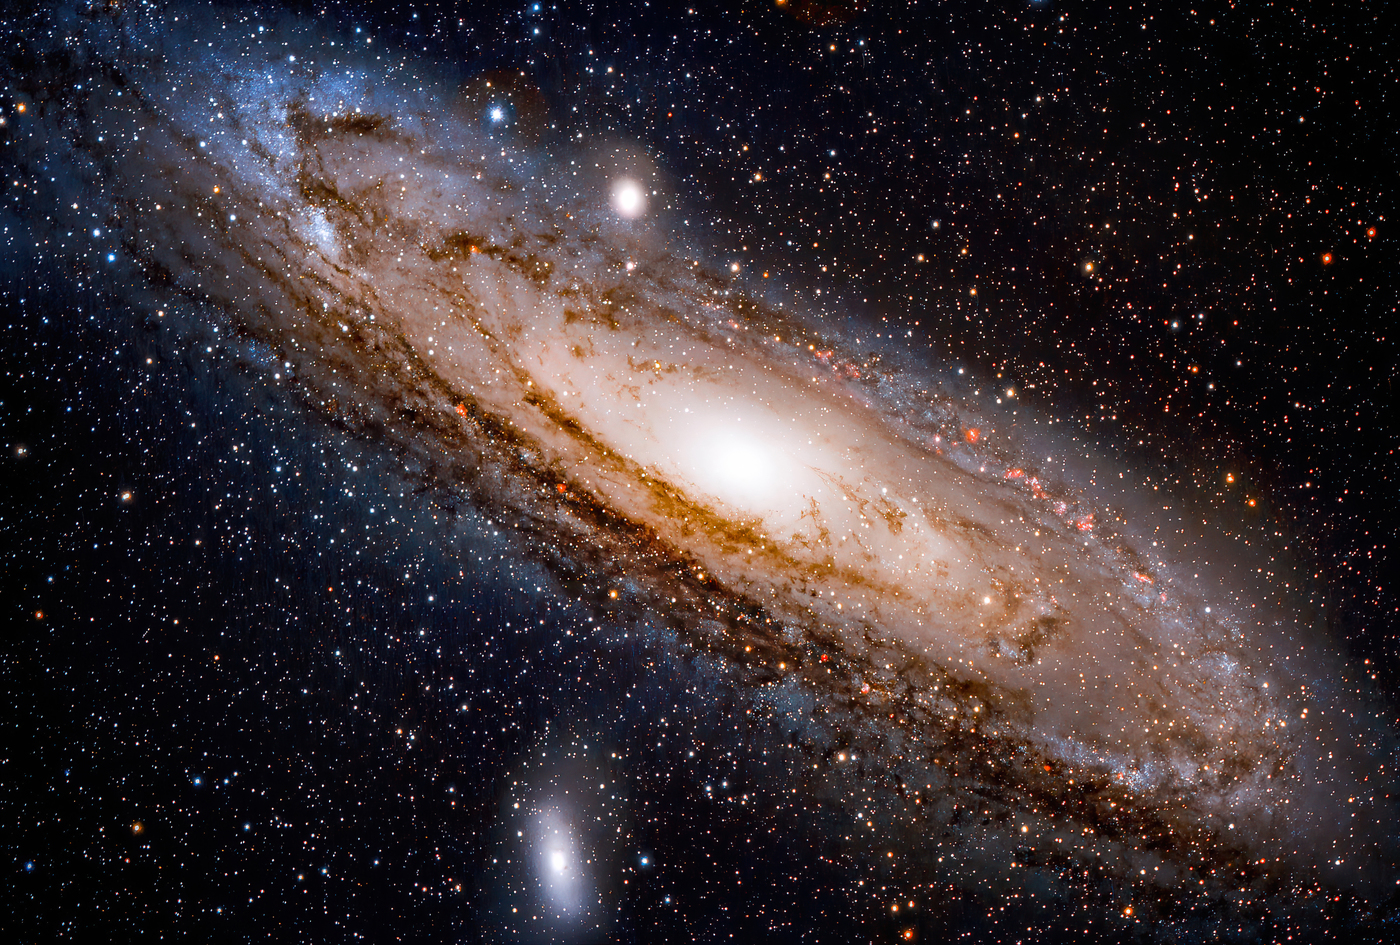
\includegraphics[width=\columnwidth]{images/M31.jpg}\caption{Andromeda galaxy (М31)}\end{figure}}
\vs p012 2:3 In the not\hyp{}distant future, new telescopes\fnst{\textbf{new telescopes}, According to \cite{Baker1} the ``new'' 200\hyp{}inch telescope Hale, sponsored by the Rockefeller Foundation in 1928 is meant here. It was being built from 1936 until 1948.} will reveal to the wondering gaze of Urantian astronomers no less than 375,000,000 new galaxies in the remote stretches of outer space. At the same time these more powerful telescopes will disclose that many island universes formerly believed to be in outer space are really a part of the galactic system of Orvonton. The seven superuniverses are still growing; the periphery of each is gradually expanding; new nebulae are constantly being stabilized and organized; and some of the nebulae which Urantian astronomers regard as extragalactic are actually on the fringe of Orvonton and are travelling along with us.\fnst{\textbf{travelling along with us}, Perhaps the Large and Small Magellanic Clouds are meant here.}\tunemarkup{pictures}{\begin{figure}[H]\centering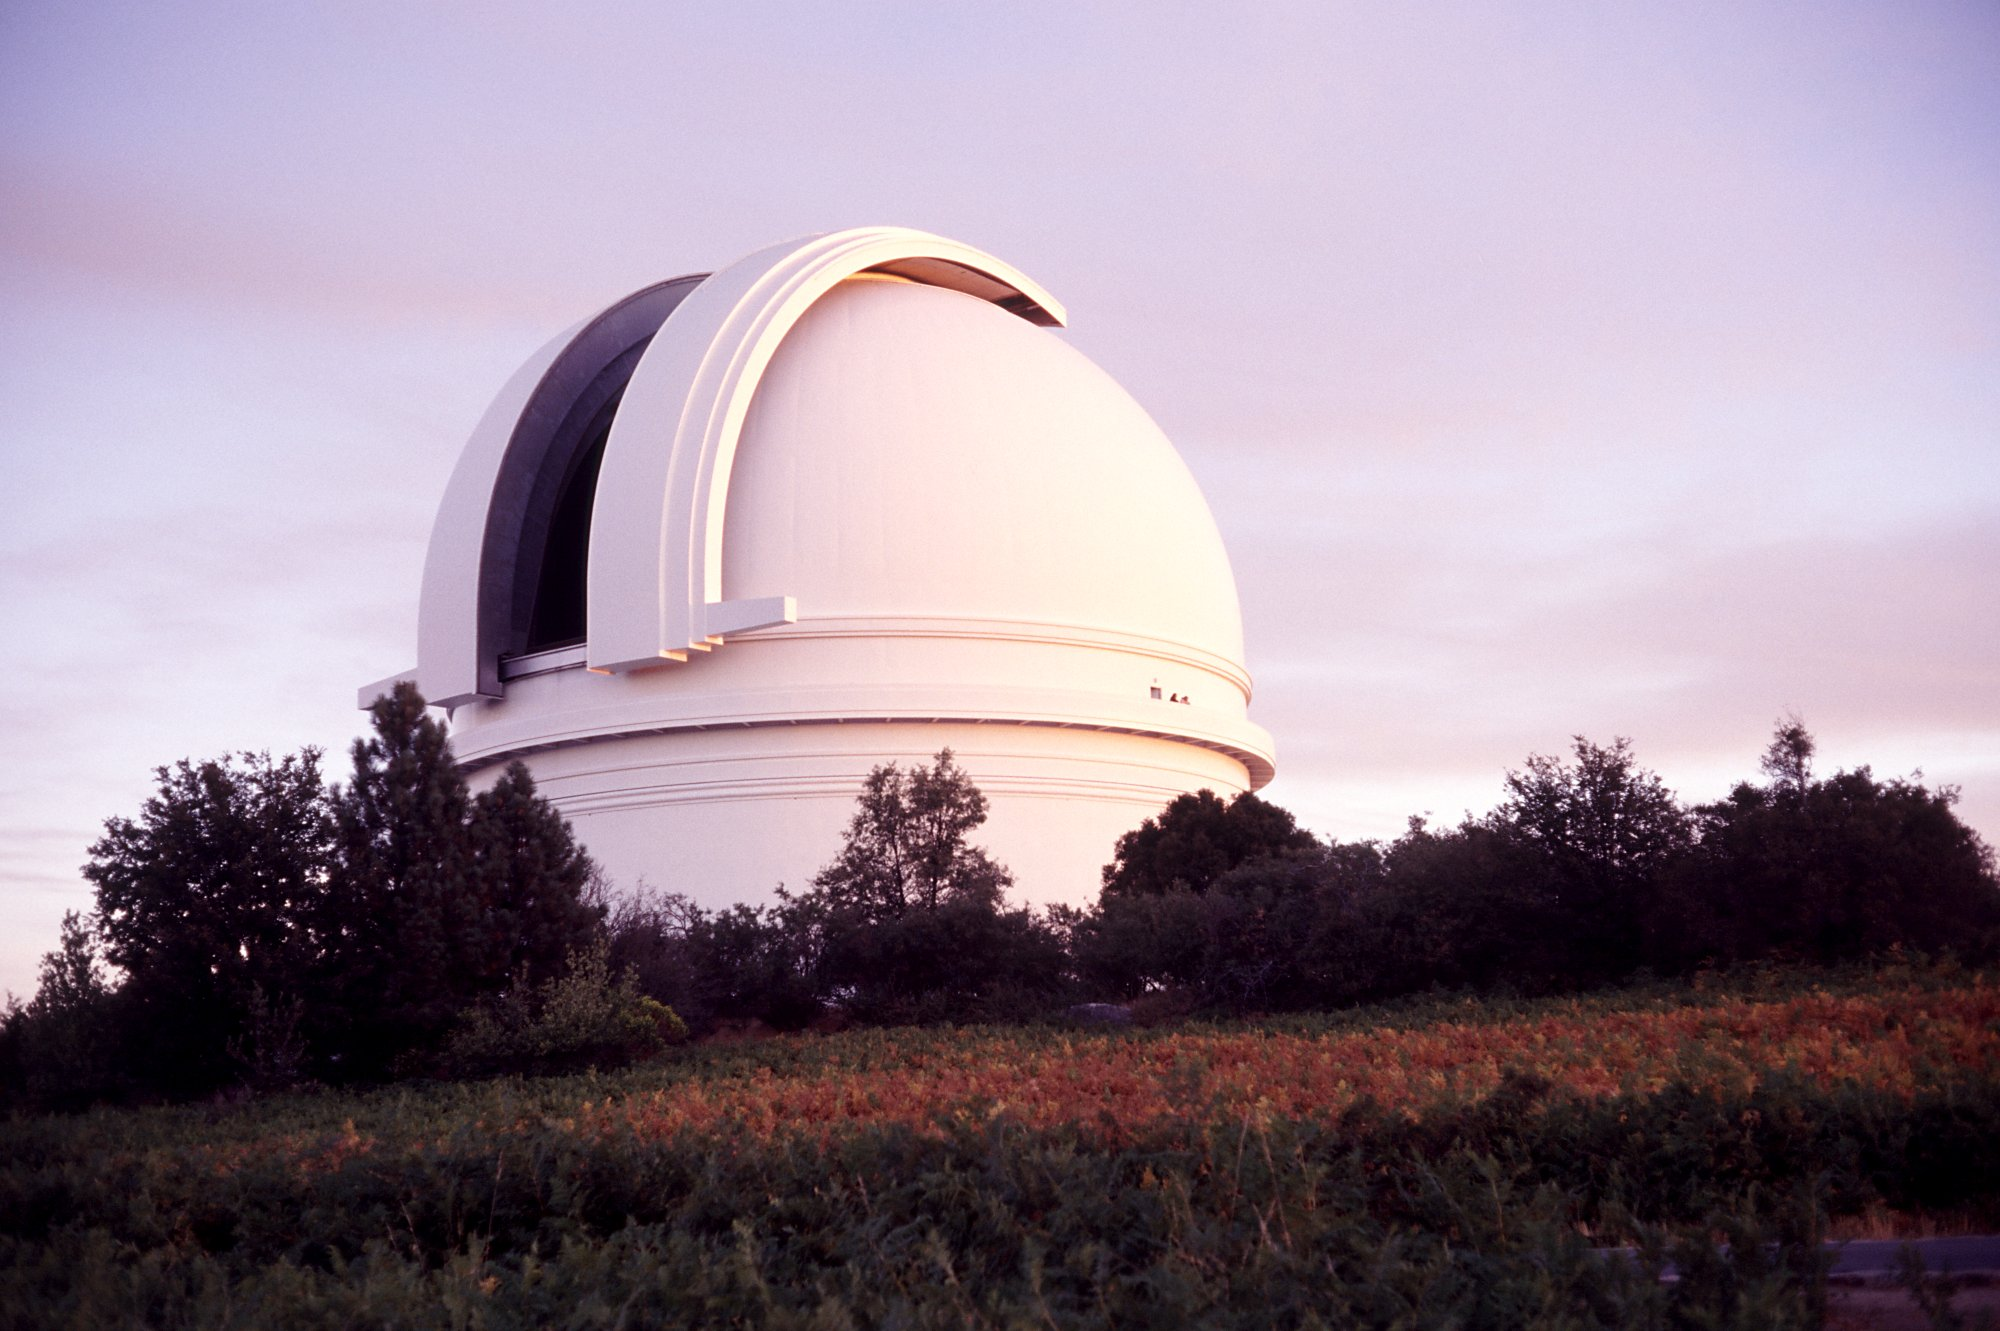
\includegraphics[width=\columnwidth]{images/Hale-200inch.jpg}\caption{200\hyp{}inch telescope George Ellery Hale in San Diego, California, USA}\end{figure}}
\vs p012 2:4 \pc The Uversa star students observe that the grand universe is surrounded by the ancestors of a series of starry and planetary clusters which completely encircle the present inhabited creation as concentric rings of outer universes upon universes. The physicists of Uversa calculate that the energy and matter of these outer and uncharted regions already equal many times the total material mass and energy charge embraced in all seven superuniverses. We are informed that the metamorphosis of cosmic force in these outer space levels is a function of the Paradise force organizers. We also know that these forces are ancestral to those physical energies which at present activate the grand universe. The Orvonton power directors, however, have nothing to do with these far\hyp{}distant realms, neither are the energy movements therein discernibly connected with the power circuits of the organized and inhabited creations.\tunemarkup{pictures}{\begin{figure}[H]\centering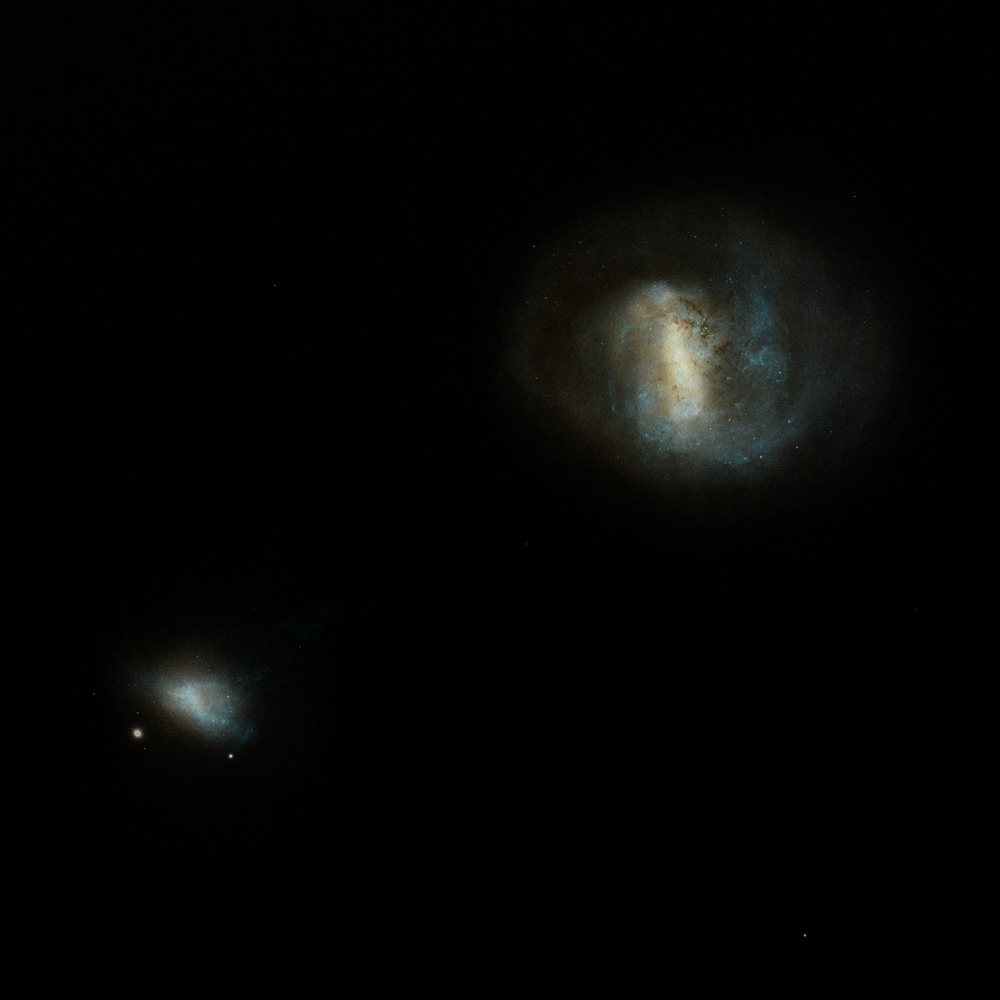
\includegraphics[width=\columnwidth]{images/LMC.jpg}\caption{Large and Small Magellanic Clouds}\end{figure}}
\vs p012 2:5 \pc We know very little of the significance of these tremendous phenomena of outer space. A greater creation of the future is in process of formation. We can observe its immensity, we can discern its extent and sense its majestic dimensions, but otherwise we know little more about these realms than do the astronomers of Urantia. As far as we know, no material beings on the order of humans, no angels or other spirit creatures, exist in this outer ring of nebulae, suns, and planets. This distant domain is beyond the jurisdiction and administration of the superuniverse governments.
\vs p012 2:6 Throughout Orvonton it is believed that a new type of creation is in process, an order of universes destined to become the scene of the future activities of the assembling Corps of the Finality; and if our conjectures are correct, then the endless future may hold for all of you the same enthralling spectacles that the endless past has held for your seniors and predecessors.
\usection{Universal Gravity}
\vs p012 3:1 All forms of force\hyp{}energy --- material, mindal, or spiritual --- are alike subject to those grasps, those universal presences, which we call gravity. Personality also is responsive to gravity --- to the Father’s exclusive circuit; but though this circuit is exclusive to the Father, he is not excluded from the other circuits; the Universal Father is infinite and acts over \bibemph{all} four absolute\hyp{}gravity circuits in the master universe:
\vs p012 3:2 \ublistelem{1.}\bibnobreakspace The Personality Gravity of the Universal Father.
\vs p012 3:3 \ublistelem{2.}\bibnobreakspace The Spirit Gravity of the Eternal Son.
\vs p012 3:4 \ublistelem{3.}\bibnobreakspace The Mind Gravity of the Conjoint Actor.
\vs p012 3:5 \ublistelem{4.}\bibnobreakspace The Cosmic Gravity of the Isle of Paradise.
\vs p012 3:6 \pc These four circuits are not related to the nether Paradise force centre; they are neither force, energy, nor power circuits. They are absolute \bibemph{presence} circuits and like God are independent of time and space.
\vs p012 3:7 In this connection it is interesting to record certain observations made on Uversa during recent millenniums by the corps of gravity researchers. This expert group of workers has arrived at the following conclusions regarding the different gravity systems of the master universe:
\vs p012 3:8 \ublistelem{1.}\bibnobreakspace \bibemph{Physical Gravity.} Having formulated an estimate of the summation of the entire physical\hyp{}gravity capacity of the grand universe, they have laboriously effected a comparison of this finding with the estimated total of absolute gravity presence now operative. These calculations indicate that the total gravity action on the grand universe is a very small part of the estimated gravity pull of Paradise, computed on the basis of the gravity response of basic physical units of universe matter. These investigators reach the amazing conclusion that the central universe and the surrounding seven superuniverses are at the present time making use of only about 5\% of the active functioning of the Paradise absolute\hyp{}gravity grasp. In other words: At the present moment about 95\% of the active cosmic\hyp{}gravity action of the Isle of Paradise, computed on this totality theory, is engaged in controlling material systems beyond the borders of the present organized universes. These calculations all refer to absolute gravity; linear gravity is an interactive phenomenon which can be computed only by knowing the actual Paradise gravity.
\vs p012 3:9 \ublistelem{2.}\bibnobreakspace \bibemph{Spiritual Gravity.} By the same technique of comparative estimation and calculation these researchers have explored the present reaction capacity of spirit gravity and, with the co\hyp{}operation of Solitary Messengers and other spirit personalities, have arrived at the summation of the active spirit gravity of the Second Source and Centre. And it is most instructive to note that they find about the same value for the actual and functional presence of spirit gravity in the grand universe that they postulate for the present total of active spirit gravity. In other words: At the present time practically the entire spirit gravity of the Eternal Son, computed on this theory of totality, is observable as functioning in the grand universe. If these findings are dependable, we may conclude that the universes now evolving in outer space are at the present time wholly nonspiritual. And if this is true, it would satisfactorily explain why spirit\hyp{}endowed beings are in possession of little or no information about these vast energy manifestations aside from knowing the fact of their physical existence.
\vs p012 3:10 \ublistelem{3.}\bibnobreakspace \bibemph{Mind Gravity.} By these same principles of comparative computation these experts have attacked the problem of mind\hyp{}gravity presence and response. The mind unit of estimation was arrived at by averaging three material and three spiritual types of mentality, although the type of mind found in the power directors and their associates proved to be a disturbing factor in the effort to arrive at a basic unit for mind\hyp{}gravity estimation. There was little to impede the estimation of the present capacity of the Third Source and Centre for mind\hyp{}gravity function in accordance with this theory of totality. Although the findings in this instance are not so conclusive as in the estimates of physical and spirit gravity, they are, comparatively considered, very instructive, even intriguing. These investigators deduce that about 85\% of the mind\hyp{}gravity response to the intellectual drawing of the Conjoint Actor takes origin in the existing grand universe. This would suggest the possibility that mind activities are involved in connection with the observable physical activities now in progress throughout the realms of outer space. While this estimate is probably far from accurate, it accords, in principle, with our belief that intelligent force organizers are at present directing universe evolution in the space levels beyond the present outer limits of the grand universe. Whatever the nature of this postulated intelligence, it is apparently not spirit\hyp{}gravity responsive.
\vs p012 3:11 But all these computations are at best estimates based on assumed laws. We think they are fairly reliable. Even if a few spirit beings were located in outer space, their collective presence would not markedly influence calculations involving such enormous measurements.
\vs p012 3:12 \pc \bibemph{Personality Gravity} is noncomputable. We recognize the circuit, but we cannot measure either qualitative or quantitative realities responsive thereto.
\usection{Space and Motion}
\vs p012 4:1 All units of cosmic energy are in primary revolution, are engaged in the execution of their mission, while swinging around the universal orbit. The universes of space and their component systems and worlds are all revolving spheres, moving along the endless circuits of the master universe space levels. Absolutely nothing is stationary in all the master universe except the very centre of Havona, the eternal Isle of Paradise, the centre of gravity.
\vs p012 4:2 The Unqualified Absolute is functionally limited to space, but we are not so sure about the relation of this Absolute to motion. Is motion inherent therein? We do not know. We know that motion is not inherent in space; even the motions \bibemph{of} space are not innate. But we are not so sure about the relation of the Unqualified to motion. Who, or what, is really responsible for the gigantic activities of force\hyp{}energy transmutations now in progress out beyond the borders of the present seven superuniverses? Concerning the origin of motion we have the following opinions:
\vs p012 4:3 \ublistelem{1.}\bibnobreakspace We think the Conjoint Actor initiates motion \bibemph{in} space.
\vs p012 4:4 \ublistelem{2.}\bibnobreakspace If the Conjoint Actor produces the motions \bibemph{of} space, we cannot prove it.
\vs p012 4:5 \ublistelem{3.}\bibnobreakspace The Universal Absolute does not originate initial motion but does equalize and control all of the tensions originated by motion.
\vs p012 4:6 \pc In outer space the force organizers are apparently responsible for the production of the gigantic universe wheels which are now in process of stellar evolution, but their ability so to function must have been made possible by some modification of the space presence of the Unqualified Absolute.
\vs p012 4:7 \pc Space is, from the human viewpoint, nothing --- negative; it exists only as related to something positive and nonspatial. Space is, however, real. It contains and conditions motion. It even moves. Space motions may be roughly classified as follows:
\vs p012 4:8 \ublistelem{1.}\bibnobreakspace Primary motion --- space respiration, the motion of space itself.
\vs p012 4:9 \ublistelem{2.}\bibnobreakspace Secondary motion --- the alternate directional swings of the successive space levels.
\vs p012 4:10 \ublistelem{3.}\bibnobreakspace Relative motions --- relative in the sense that they are not evaluated with Paradise as a base point. Primary and secondary motions are absolute, motion in relation to unmoving Paradise.
\vs p012 4:11 \ublistelem{4.}\bibnobreakspace Compensatory or correlating movement designed to co\hyp{}ordinate all other motions.
\vs p012 4:12 \pc The present relationship of your sun and its associated planets, while disclosing many relative and absolute motions in space, tends to convey the impression to astronomic observers that you are comparatively stationary in space, and that the surrounding starry clusters and streams are engaged in outward flight at ever\hyp{}increasing velocities as your calculations proceed outward in space. But such is not the case. You fail to recognize the present outward and uniform expansion of the physical creations of all pervaded space. Your own local creation (Nebadon) participates in this movement of universal outward expansion. The entire seven superuniverses participate in the two\hyp{}billion\hyp{}year cycles of space respiration along with the outer regions of the master universe.
\vs p012 4:13 When the universes expand and contract, the material masses in pervaded space alternately move against and with the pull of Paradise gravity. The work that is done in moving the material energy mass of creation is \bibemph{space} work but not \bibemph{power\hyp{}energy} work.
\vs p012 4:14 \pc Although your spectroscopic estimations of astronomic velocities are fairly reliable when applied to the starry realms belonging to your superuniverse and its associate superuniverses, such reckonings with reference to the realms of outer space are wholly unreliable. Spectral lines are displaced from the normal towards the violet by an approaching star; likewise these lines are displaced towards the red by a receding star. Many influences interpose to make it appear that the recessional velocity of the external universes increases at the rate of more than 160 km/s for every 1,000,000 light\hyp{}years\fnst{The value of Hubble constant given in the text (522\,km/s/Mpc) is very close to the value obtained by Hubble himself in 1935: 535\,km/s/Mpc. Hubble's calculations were based on the dependence between the period and luminosity of variable stars called Cepheids. The revision of the base point of this dependence by W.~Baade in 1952 led to the significant correction of the value of Hubble's constant. By 1955 the accepted value became 180\,km/s/Mpc and the modern (2016) value is even smaller: 6,93$\pm$0,62\,km/s/Mpc.} increase in distance. By this method of reckoning, subsequent to the perfection of more powerful telescopes, it will appear that these far\hyp{}distant systems are in flight from this part of the universe at the unbelievable rate of more than 48,000 km/s. But this apparent speed of recession is not real; it results from numerous factors of error embracing angles of observation and other time\hyp{}space distortions.
\vs p012 4:15 But the greatest of all such distortions arises because the vast universes of outer space, in the realms\fnc{\textbf{outer space, in the realms}, In 1955 text no comma.} next to the domains of the seven superuniverses, seem to be revolving in a direction opposite to that of the grand universe. That is, these myriads of nebulae and their accompanying suns and spheres are at the present time revolving clockwise about the central creation. The seven superuniverses revolve about Paradise in a counterclockwise direction. It appears that the second outer universe of galaxies, like the seven superuniverses, revolves counterclockwise about Paradise. And the astronomic observers of Uversa think they detect evidence of revolutionary movements in a third outer belt of far\hyp{}distant space which are beginning to exhibit directional tendencies of a clockwise nature.
\vs p012 4:16 It is probable that these alternate directions of successive space processions of the universes have something to do with the intramaster universe gravity technique of the Universal Absolute, which consists of a co\hyp{}ordination of forces and an equalization of space tensions. Motion as well as space is a complement or equilibrant of gravity.
\usection{Space and Time}
\vs p012 5:1 Like space, time is a bestowal of Paradise, but not in the same sense, only indirectly. Time comes by virtue of motion and because mind is inherently aware of sequentiality. From a practical viewpoint, motion is essential to time, but there is no universal time unit based on motion except in so far as the Paradise\hyp{}Havona standard day is arbitrarily so recognized. The totality of space respiration destroys its local value as a time source.
\vs p012 5:2 Space is not infinite, even though it takes origin from Paradise; not absolute, for it is pervaded by the Unqualified Absolute. We do not know the absolute limits of space, but we do know that the absolute of time is eternity.
\vs p012 5:3 \pc Time and space are inseparable only in the time\hyp{}space creations, the seven superuniverses. Nontemporal space (space without time) theoretically exists, but the only truly nontemporal place is Paradise \bibemph{area.} Nonspatial time (time without space) exists in mind of the Paradise level of function.
\vs p012 5:4 The relatively motionless midspace zones impinging on Paradise and separating pervaded from unpervaded space are the transition zones from time to eternity, hence the necessity of Paradise pilgrims becoming unconscious during this transit when it is to culminate in Paradise citizenship. Time\hyp{}conscious \bibemph{visitors} can go to Paradise without thus sleeping, but they remain creatures of time.
\vs p012 5:5 \pc Relationships to time do not exist without motion in space, but consciousness of time does. Sequentiality can consciousize time even in the absence of motion. Man’s mind is less time\hyp{}bound than space\hyp{}bound because of the inherent nature of mind. Even during the days of the earth life in the flesh, though man’s mind is rigidly space\hyp{}bound, the creative human imagination is comparatively time free. But time itself is not genetically a quality of mind.
\vs p012 5:6 \pc There are three different levels of time cognizance:
\vs p012 5:7 \ublistelem{1.}\bibnobreakspace Mind\hyp{}perceived time --- consciousness of sequence, motion, and a sense of duration.
\vs p012 5:8 \ublistelem{2.}\bibnobreakspace Spirit\hyp{}perceived time --- insight into motion Godward and the awareness of the motion of ascent to levels of increasing divinity.
\vs p012 5:9 \ublistelem{3.}\bibnobreakspace Personality \bibemph{creates} a unique time sense out of insight into Reality plus a consciousness of presence and an awareness of duration.
\vs p012 5:10 \pc Unspiritual animals know only the past and live in the present. Spirit\hyp{}indwelt man has powers of prevision (insight); he may visualize the future. Only forward\hyp{}looking and progressive attitudes are personally real. Static ethics and traditional morality are just slightly superanimal. Nor is stoicism a high order of self\hyp{}realization. Ethics and morals become truly human when they are dynamic and progressive, alive with universe reality.
\vs p012 5:11 The human personality is not merely a concomitant of time\hyp{}and\hyp{}space events; the human personality can also act as the cosmic cause of such events.
\usection{Universal Overcontrol}
\vs p012 6:1 The universe is nonstatic. Stability is not the result of inertia but rather the product of balanced energies, co\hyp{}operative minds, co\hyp{}ordinated morontias, spirit overcontrol, and personality unification. Stability is wholly and always proportional to divinity.
\vs p012 6:2 In the physical control of the master universe the Universal Father exercises priority and primacy through the Isle of Paradise; God is absolute in the spiritual administration of the cosmos in the person of the Eternal Son. Concerning the domains of mind, the Father and the Son function co\hyp{}ordinately in the Conjoint Actor.
\vs p012 6:3 The Third Source and Centre assists in the maintenance of the equilibrium and co\hyp{}ordination of the combined physical and spiritual energies and organizations by the absoluteness of his grasp of the cosmic mind and by the exercise of his inherent and universal physical\hyp{} and spiritual\hyp{}gravity complements. Whenever and wherever there occurs a liaison between the material and the spiritual, such a mind phenomenon is an act of the Infinite Spirit. Mind alone can interassociate the physical forces and energies of the material level with the spiritual powers and beings of the spirit level.
\vs p012 6:4 In all your contemplation of universal phenomena, make certain that you take into consideration the interrelation of physical, intellectual, and spiritual energies, and that due allowance is made for the unexpected phenomena attendant upon their unification by personality and for the unpredictable phenomena resulting from the actions and reactions of experiential Deity and the Absolutes.
\vs p012 6:5 The universe is highly predictable only in the quantitative or gravity\hyp{}measurement sense; even the primal physical forces are not responsive to linear gravity, nor are the higher mind meanings and true spirit values of ultimate universe realities. Qualitatively, the universe is not highly predictable as regards new associations of forces, either physical, mindal, or spiritual, although many such combinations of energies or forces become partially predictable when subjected to critical observation. When matter, mind, and spirit are unified by creature personality, we are unable fully to predict the decisions of such a freewill being.
\vs p012 6:6 \pc All phases of primordial force, nascent spirit, and other nonpersonal ultimates appear to react in accordance with certain relatively stable but unknown laws and are characterized by a latitude of performance and an elasticity of response which are often disconcerting when encountered in the phenomena of a circumscribed and isolated situation. What is the explanation of this unpredictable freedom of reaction disclosed by these emerging universe actualities? These unknown, unfathomable unpredictables --- whether pertaining to the behaviour of a primordial unit of force, the reaction of an unidentified level of mind, or the phenomenon of a vast preuniverse in the making in the domains of outer space --- probably disclose the activities of the Ultimate and the presence\hyp{}performances of the Absolutes, which antedate the function of all universe Creators.
\vs p012 6:7 We do not really know, but we surmise that such amazing versatility and such profound co\hyp{}ordination signify the presence and performance of the Absolutes, and that such diversity of response in the face of apparently uniform causation discloses the reaction of the Absolutes, not only to the immediate and situational causation, but also to all other related causations throughout the entire master universe.
\vs p012 6:8 \pc Individuals have their guardians of destiny; planets, systems, constellations, universes, and superuniverses each have their respective rulers who labour for the good of their domains. Havona and even the grand universe are watched over by those entrusted with such high responsibilities. But who fosters and cares for the fundamental needs of the master universe as a whole, from Paradise to the fourth and outermost space level? Existentially such overcare is probably attributable to the Paradise Trinity, but from an experiential viewpoint the appearance of the post\hyp{}Havona universes is dependent on:
\vs p012 6:9 \ublistelem{1.}\bibnobreakspace The Absolutes in potential.
\vs p012 6:10 \ublistelem{2.}\bibnobreakspace The Ultimate in direction.
\vs p012 6:11 \ublistelem{3.}\bibnobreakspace The Supreme in evolutionary co\hyp{}ordination.
\vs p012 6:12 \ublistelem{4.}\bibnobreakspace The Architects of the Master Universe in administration prior to the appearance of specific rulers.
\vs p012 6:13 \pc The Unqualified Absolute pervades all space. We are not altogether clear as to the exact status of the Deity and Universal Absolutes, but we know the latter functions wherever the Deity and Unqualified Absolutes function. The Deity Absolute may be universally present but hardly space present. The Ultimate is, or sometime will be, space present to the outer margins of the fourth space level. We doubt that the Ultimate will ever have a space presence beyond the periphery of the master universe, but within this limit the Ultimate is progressively integrating the creative organization of the potentials of the three Absolutes.
\usection{The Part and the Whole}
\vs p012 7:1 There is operative throughout all time and space and with regard to all reality of whatever nature an inexorable and impersonal law which is equivalent to the function of a cosmic providence. Mercy characterizes God’s attitude of love for the individual; impartiality motivates God’s attitude toward the total. The will of God does not necessarily prevail in the part --- the heart of any one personality --- but his will does actually rule the whole, the universe of universes.
\vs p012 7:2 \pc In all his dealings with all his beings it is true that the laws of God are not inherently arbitrary. To you, with your limited vision and finite viewpoint, the acts of God must often appear to be dictatorial and arbitrary. The laws of God are merely the habits of God\fnst{\textbf{The laws of God are merely the habits of God}, This thought comes from \cite{Strong1}.}, his way of repeatedly doing things; and he ever does all things well. You observe that God does the same thing in the same way, repeatedly, simply because that is the best way to do that particular thing in a given circumstance; and the best way is the right way, and therefore does infinite wisdom always order it done in that precise and perfect manner. You should also remember that nature is not the exclusive act of Deity; other influences are present in those phenomena which man calls nature.
\vs p012 7:3 It is repugnant to the divine nature to suffer any sort of deterioration or ever to permit the execution of any purely personal act in an inferior way. It should be made clear, however, that, \bibemph{if,} in the divinity of any situation, in the extremity of any circumstance, in any case where the course of supreme wisdom might indicate the demand for different conduct --- if the demands of perfection might for any reason dictate another method of reaction, a better one, then and there would the all\hyp{}wise God function in that better and more suitable way. That would be the expression of a higher law, not the reversal of a lower law.
\vs p012 7:4 God is not a habit\hyp{}bound slave to the chronicity of the repetition of his own voluntary acts. There is no conflict among the laws of the Infinite; they are all perfections of the infallible nature; they are all the unquestioned acts expressive of faultless decisions. Law is the unchanging reaction of an infinite, perfect, and divine mind. The acts of God are all volitional notwithstanding this apparent sameness. In God there “is no variableness neither shadow of changing.”\fnst{See James~1:17.} But all this which can be truly said of the Universal Father cannot be said with equal certainty of all his subordinate intelligences or of his evolutionary creatures.
\vs p012 7:5 Because God is changeless, therefore can you depend, in all ordinary circumstances, on his doing the same thing in the same identical and ordinary way. God is the assurance of stability for all created things and beings. He is God; therefore he changes not.
\vs p012 7:6 And all this steadfastness of conduct and uniformity of action is personal, conscious, and highly volitional, for the great God is not a helpless slave to his own perfection and infinity. God is not a self\hyp{}acting automatic force; he is not a slavish law\hyp{}bound power. God is neither a mathematical equation nor a chemical formula. He is a freewill and primal personality. He is the Universal Father, a being surcharged with personality and the universal fount of all creature personality.
\vs p012 7:7 \pc The will of God does not uniformly prevail in the heart of the God\hyp{}seeking material mortal, but if the time frame is enlarged beyond the moment to embrace the whole of the first life, then does God’s will become increasingly discernible in the spirit fruits which are borne in the lives of the spirit\hyp{}led children of God. And then, if human life is further enlarged to include the morontia experience, the divine will is observed to shine brighter and brighter in the spiritualizing acts of those creatures of time who have begun to taste the divine delights of experiencing the relationship of the personality of man with the personality of the Universal Father.
\vs p012 7:8 The Fatherhood of God and the brotherhood of man present the paradox of the part and the whole on the level of personality. God loves \bibemph{each} individual as an individual child in the heavenly family. Yet God thus loves \bibemph{every} individual; he is no respecter of persons, and the universality of his love brings into being a relationship of the whole, the universal brotherhood.
\vs p012 7:9 The love of the Father absolutely individualizes each personality as a unique child of the Universal Father, a child without duplicate in infinity, a will creature irreplaceable in all eternity. The Father’s love glorifies each child of God, illuminating each member of the celestial family, sharply silhouetting the unique nature of each personal being against the impersonal levels that lie outside the fraternal circuit of the Father of all. The love of God strikingly portrays the transcendent value of each will creature, unmistakably reveals the high value which the Universal Father has placed upon each and every one of his children from the highest creator personality of Paradise status to the lowest personality of will dignity among the savage tribes of men in the dawn of the human species on some evolutionary world of time and space.
\vs p012 7:10 This very love of God for the individual brings into being the divine family of all individuals, the universal brotherhood of the freewill children of the Paradise Father. And this brotherhood, being universal, is a relationship of the whole. Brotherhood, when universal, discloses not the \bibemph{each} relationship, but the \bibemph{all} relationship. Brotherhood is a reality of the total and therefore discloses qualities of the whole in contradistinction to qualities of the part.
\vs p012 7:11 Brotherhood constitutes a fact of relationship between every personality in universal existence. No person can escape the benefits or the penalties that may come as a result of relationship to other persons. The part profits or suffers in measure with the whole. The good effort of each man benefits all men; the error or evil of each man augments the tribulation of all men. As moves the part, so moves the whole. As the progress of the whole, so the progress of the part. The relative velocities of part and whole determine whether the part is retarded by the inertia of the whole or is carried forward by the momentum of the cosmic brotherhood.
\vs p012 7:12 \pc It is a mystery that God is a highly personal self\hyp{}conscious being with residential headquarters, and at the same time personally present in such a vast universe and personally in contact with such a well\hyp{}nigh infinite number of beings. That such a phenomenon is a mystery beyond human comprehension should not in the least lessen your faith. Do not allow the magnitude of the infinity, the immensity of the eternity, and the grandeur and glory of the matchless character of God to overawe, stagger, or discourage you; for the Father is not very far from any one of you; he dwells within you, and in him do we all literally move, actually live, and veritably have our being.
\vs p012 7:13 \pc Even though the Paradise Father functions through his divine creators and his creature children, he also enjoys the most intimate inner contact with you, so sublime, so highly personal, that it is even beyond my comprehension --- that mysterious communion of the Father fragment with the human soul and with the mortal mind of its actual indwelling. Knowing what you do of these gifts of God, you therefore know that the Father is in intimate touch, not only with his divine associates, but also with his evolutionary mortal children of time. The Father indeed abides on Paradise, but his divine presence also dwells in the minds of men.
\vs p012 7:14 Even though the spirit of a Son be poured out upon all flesh, even though a Son once dwelt with you in the likeness of mortal flesh, even though the seraphim personally guard and guide you, how can any of these divine beings of the Second and Third Centres ever hope to come as near to you or to understand you as fully as the Father, who has given a part of himself to be in you, to be your real and divine, even your eternal, self?
\usection{Matter, Mind, and Spirit}
\vs p012 8:1 “God is spirit,” but Paradise is not. The material universe is always the arena wherein take place all spiritual activities; spirit beings and spirit ascenders live and work on physical spheres of material reality.
\vs p012 8:2 \pc The bestowal of cosmic force, the domain of cosmic gravity, is the function of the Isle of Paradise. All original force\hyp{}energy proceeds from Paradise, and the matter for the making of untold universes now circulates throughout the master universe in the form of a supergravity presence which constitutes the force\hyp{}charge of pervaded space.
\vs p012 8:3 Whatever the transformations of force in the outlying universes, having gone out from Paradise, it journeys on subject to the never\hyp{}ending, ever\hyp{}present, unfailing pull of the eternal Isle, obediently and inherently swinging on forever around the eternal space paths of the universes. Physical energy is the one reality which is true and steadfast in its obedience to universal law. Only in the realms of creature volition has there been deviation from the divine paths and the original plans. Power and energy are the universal evidences of the stability, constancy, and eternity of the central Isle of Paradise.
\vs p012 8:4 \pc The bestowal of spirit and the spiritualization of personalities, the domain of spiritual gravity, is the realm of the Eternal Son. And this spirit gravity of the Son, ever drawing all spiritual realities to himself, is just as real and absolute as is the all\hyp{}powerful material grasp of the Isle of Paradise. But material\hyp{}minded man is naturally more familiar with the material manifestations of a physical nature than with the equally real and mighty operations of a spiritual nature which are discerned only by the spiritual insight of the soul.
\vs p012 8:5 As the mind of any personality in the universe becomes more spiritual --- Godlike --- it becomes less responsive to material gravity. Reality, measured by physical\hyp{}gravity response, is the antithesis of reality as determined by quality of spirit content. Physical\hyp{}gravity action is a quantitative determiner of nonspirit energy; spiritual\hyp{}gravity action is the qualitative measure of the living energy of divinity.
\vs p012 8:6 \pc What Paradise is to the physical creation, and what the Eternal Son is to the spiritual universe, the Conjoint Actor is to the realms of mind --- the intelligent universe of material, morontial, and spiritual beings and personalities.
\vs p012 8:7 The Conjoint Actor reacts to both material and spiritual realities and therefore inherently becomes the universal minister to all intelligent beings, beings who may represent a union of both the material and spiritual phases of creation. The endowment of intelligence, the ministry to the material and the spiritual in the phenomenon of mind, is the exclusive domain of the Conjoint Actor, who thus becomes the partner of the spiritual mind, the essence of the morontia mind, and the substance of the material mind of the evolutionary creatures of time.
\vs p012 8:8 Mind is the technique whereby spirit realities become experiential to creature personalities. And in the last analysis the unifying possibilities of even human mind, the ability to co\hyp{}ordinate things, ideas, and values, is supermaterial.
\vs p012 8:9 \pc Though it is hardly possible for the mortal mind to comprehend the seven levels of relative cosmic reality, the human intellect should be able to grasp much of the meaning of three functioning levels of finite reality:
\vs p012 8:10 \ublistelem{1.}\bibnobreakspace \bibemph{Matter.} Organized energy which is subject to linear gravity except as it is modified by motion and conditioned by mind.
\vs p012 8:11 \ublistelem{2.}\bibnobreakspace \bibemph{Mind.} Organized consciousness which is not wholly subject to material gravity, and which becomes truly liberated when modified by spirit.
\vs p012 8:12 \ublistelem{3.}\bibnobreakspace \bibemph{Spirit.} The highest personal reality. True spirit is not subject to physical gravity but eventually becomes the motivating influence of all evolving energy systems of personality dignity.
\vs p012 8:13 \pc The goal of existence of all personalities is spirit; material manifestations are relative, and the cosmic mind intervenes between these universal opposites. The bestowal of mind and the ministration of spirit are the work of the associate persons of Deity, the Infinite Spirit and the Eternal Son. Total Deity reality is not mind but spirit\hyp{}mind --- mind\hyp{}spirit unified by personality. Nevertheless the absolutes of both the spirit and the thing converge in the person of the Universal Father.
\vs p012 8:14 \pc On Paradise the three energies, physical, mindal, and spiritual, are co\hyp{}ordinate. In the evolutionary cosmos energy\hyp{}matter is dominant except in personality, where spirit, through the mediation of mind, is striving for the mastery. Spirit is the fundamental reality of the personality experience of all creatures because God is spirit. Spirit is unchanging, and therefore, in all personality relations, it transcends both mind and matter, which are experiential variables of progressive attainment.
\vs p012 8:15 In cosmic evolution matter becomes a philosophic shadow cast by mind in the presence of spirit luminosity of divine enlightenment, but this does not invalidate the reality of matter\hyp{}energy. Mind, matter, and spirit are equally real, but they are not of equal value to personality in the attainment of divinity. Consciousness of divinity is a progressive spiritual experience.
\vs p012 8:16 The brighter the shining of the spiritualized personality (the Father in the universe, the fragment of potential spirit personality in the individual creature), the greater the shadow cast by the intervening mind upon its material investment. In time, man’s body is just as real as mind or spirit, but in death, both mind (identity) and spirit survive while the body does not. A cosmic reality can be nonexistent in personality experience. And so your Greek figure of speech --- the material as the shadow of the more real spirit substance --- does have a philosophic significance.
\usection{Personal Realities}
\vs p012 9:1 Spirit is the basic personal reality in the universes, and personality is basic to all progressing experience with spiritual reality. Every phase of personality experience on every successive level of universe progression swarms with clues to the discovery of alluring personal realities. Man’s true destiny consists in the creation of new and spirit goals and then in responding to the cosmic allurements of such supernal goals of nonmaterial value.
\vs p012 9:2 \pc Love is the secret of beneficial association between personalities. You cannot really know a person as the result of a single contact. You cannot appreciatingly know music through mathematical deduction, even though music is a form of mathematical rhythm. The number assigned to a telephone subscriber does not in any manner identify the personality of that subscriber or signify anything concerning his character.
\vs p012 9:3 Mathematics\fnst{Mathematics is a creation of the material mind just like the morontia mathematics corresponds to the morontia type of mind, see \bibref[112:1.11]{p112 1:11}.}, material science, is indispensable to the intelligent discussion of the material aspects of the universe, but such knowledge is not necessarily a part of the higher realization of truth or of the personal appreciation of spiritual realities. Not only in the realms of life but even in the world of physical energy, the sum of two or more things is very often something \bibemph{more} than, or something \bibemph{different} from, the predictable additive consequences of such unions. The entire science of mathematics, the whole domain of philosophy, the highest physics or chemistry, could not predict or know that the union of two gaseous hydrogen atoms with one gaseous oxygen atom would result in a new and qualitatively superadditive substance --- liquid water. The understanding knowledge of this one physiochemical phenomenon should have prevented the development of materialistic philosophy and mechanistic cosmology.
\vs p012 9:4 Technical analysis does not reveal what a person or a thing can do. For example: Water is used effectively to extinguish fire. That water will put out fire is a fact of everyday experience, but no analysis of water could ever be made to disclose such a property. Analysis determines that water is composed of hydrogen and oxygen; a further study of these elements discloses that oxygen is the real supporter of combustion and that hydrogen will itself freely burn.
\vs p012 9:5 Your religion is becoming real because it is emerging from the slavery of fear and the bondage of superstition. Your philosophy struggles for emancipation from dogma and tradition. Your science is engaged in the agelong contest between truth and error while it fights for deliverance from the bondage of abstraction, the slavery of mathematics, and the relative blindness of mechanistic materialism.
\vs p012 9:6 \pc Mortal man has a spirit nucleus. The mind is a personal\hyp{}energy system existing around a divine spirit nucleus and functioning in a material environment. Such a living relationship of personal mind and spirit constitutes the universe potential of eternal personality. Real trouble, lasting disappointment, serious defeat, or inescapable death can come only after self\hyp{}concepts presume fully to displace the governing power of the central spirit nucleus, thereby disrupting the cosmic scheme of personality identity.
\vsetoff
\vs p012 9:7 [Presented by a Perfector of Wisdom acting by authority of the Ancients of Days.]
\quizlink
\begin{thebibliography}{100}
\bibitem{Baker1}
Robert H. Baker, Ph.D.
{<<The Universe Unfolding: A Story of Man's Increasing Comprehension of the Universe Around Him.>>}
{\em Baltimore: The Williams \&\ Wilkins Company}, 1932.
\bibitem{Strong1}
Rev.~Josiah Strong, D.D.
{<<The New World\hyp{}Religion.>>}
{\em Garden City, New York: Doubleday, Page \& Company}, 1915.
\bibitem{Overstreet1}
H.A. Overstreet
{<<The Enduring Quest: A Search for a Philosophy of Life>>.}
{\em New York: W. Norton \&\ Company, Inc.}, 1931.
\end{thebibliography}
